% Topological Solitons of a Hyperelastic Vacuum
% Build:  pdflatex -> bibtex -> pdflatex -> pdflatex   (see build.sh)

\documentclass[aps,prd,preprint,nofootinbib,longbibliography]{revtex4-2}

\usepackage{amsmath}
\usepackage{amssymb}
\usepackage{bm}
\usepackage{graphicx}
\usepackage[colorlinks=true,linkcolor=blue,citecolor=blue,urlcolor=blue]{hyperref}

\newtheorem{theorem}{Theorem}
\newcommand{\qed}{\hfill$\blacksquare$}

% preprint style otherwise stretches pages vertically around deferred floats
\raggedbottom
\newcommand{\nv}{\bm{n}}
\newcommand{\Av}{\bm{A}}
\newcommand{\Bv}{\bm{B}}
\newcommand{\Qh}{Q_H}
\newcommand{\lc}{\ell_c}
\newcommand{\Ehat}{\hat{E}}
\newcommand{\Rhat}{\hat{R}}

\begin{document}

\title{Topological Solitons of a Hyperelastic Medium}

\author{Paul Vodrazka}
\affiliation{Independent researcher}

\date{\today}

\begin{abstract}
For an isotropic hyperelastic medium carrying a director microstructure we prove
that the strain energy is \emph{exactly} the Faddeev--Skyrme energy: an
$S^2$-valued director makes the third Cauchy--Green invariant vanish identically,
so the Mooney--Rivlin truncation is exact rather than approximate and the quartic
term is the medium's second elastic constant rather than an ansatz introduced
against Derrick's theorem. The dimension count that forces this fails on any
target of dimension three or more; on the frame sector $S^3$ the sextic invariant
is admissible and we measure it at $3.7\times10^{-2}$ against $10^{-7}$ for the
director. Lattice solutions for $\Qh=1\ldots4$, obtained on a discretisation free
of the odd--even null mode that otherwise destroys topological protection,
reproduce the published spectrum to $0.6$--$1.6\%$ including all four
ground-state types and obey $E\propto|\Qh|^{0.765}$ against the
Vakulenko--Kapitanskii exponent $3/4$; the charge-one energy is reported
separately as a $2.2\%$ discrepancy with the literature. Evolving the field
equations, a $\Qh=0$ collision radiates $99.8\%$ of its rest energy and leaves
nothing, while its mirror image at $\Qh=+2$ relaxes onto the independently
minimised $\Qh=2$ soliton to $0.5\%$. We then ask what the sector cannot contain,
and answer quantitatively: generations do not arise from it. The breathing mode
is a resonance of hadronic width, $\Gamma/\omega=0.12$, where a muon requires
$3\times10^{-18}$; the collective tower has a level spacing $4.2\times10^{-6}$ of
the soliton mass, so reaching the muon needs quantum number $k\simeq7\times10^3$,
at which the rotation frequency exceeds the soliton's own deformation frequency
by a factor of $66$ and the rigid body that produced the tower no longer exists;
and enlarging the target to carry a generation label forfeits the theorem above,
since $I_3$ then fails to vanish. Two sectors are reported as constraints rather
than results. A dimensional identity fixes the ratio of director stiffness to the
metric tension $\Gamma=c^4/16\pi G$ by gravitational compactness,
$\chi=8\pi(\Rhat/\Ehat)\,r_s/R$, recasting the Planck-to-particle hierarchy as
the statement that elementary particles are not black holes; it predicts nothing
further. Forward elastic $pp$ data bound the rigidity scale,
$R_\infty\gtrsim1.0\,$fm at $95\%$ CL, stable against both the impact-parameter
profile and the saturation function; current data do not discriminate saturating
from conventional growth, and the fit returns $\rho(13\,\mathrm{TeV})=0.114$
against the measured $0.098\pm0.011$.
\end{abstract}

\maketitle

\section{Introduction}
\label{sec:intro}

Manton showed that Skyrme-type energies are naturally written through the strain
tensor of a map and its principal invariants~\cite{manton1987}. Taken literally
for a medium whose order parameter is a director rather than a frame, that
observation closes: the most general isotropic hyperelastic energy of an
$S^2$-valued director in three dimensions \emph{is} the Faddeev--Skyrme energy,
with no truncation and no freedom left over. The third Cauchy--Green invariant
vanishes identically---a consequence of the target being two-dimensional---so the
Mooney--Rivlin form is not an approximation to something longer, and the quartic
term, ordinarily introduced to defeat Derrick's theorem, is the medium's second
elastic constant. That identity is the anchor of this paper. Everything else is
either a consequence of it, a test of it, or a limit on what it can carry.

The programme is deliberately narrow: the results reported here are confined to
what can be derived, computed, or falsified.
Section~\ref{sec:elastic} proves the identity and its corollary, that the
dimension count fails on any target of dimension three or more.
Section~\ref{sec:anchoring} draws the one consequence that involves gravity, an
identity relating the director stiffness to gravitational compactness.
Section~\ref{sec:spectrum} summarises the soliton spectrum for $\Qh=1\ldots4$,
whose computation and systematics are reported in the companion
paper~\cite{lattice}, together with a diagnostic that turns out to carry physical
content: a discretisation without rigidity at the cutoff scale loses topological
protection entirely. Section~\ref{sec:frame} applies the identical machinery to
the one other admissible target, the frame $S^3$, as a concrete illustration of
what makes the director case special. Section~\ref{sec:spin} states the
spin-statistics result precisely. Section~\ref{sec:dynamics} gives annihilation
and fusion the field equations and explicit time evolution they previously
lacked. Section~\ref{sec:nogo} then asks what the sector cannot contain, and
closes the routes by which generations might have been recovered from it.
Section~\ref{sec:sm} records what the homotopy classification does and does not
supply. Section~\ref{sec:scattering} turns the finite rigidity into an
observational constraint from forward-scattering data, and
Section~\ref{sec:predictions} collects, in one table, everything the framework
commits to together with the observation that would refute each item.

One interpretive hypothesis runs underneath, and we state it here so that it can
be discounted at will. Holographic duality realises the bulk as a quantum
error-correcting code whose logical operators resist local
erasure~\cite{almheiri2015,pastawski2015}, and Sakharov's induced-gravity
argument~\cite{sakharov1967}, later sharpened by Jacobson~\cite{jacobson1995},
presents the Einstein equation as an equation of state of an underlying medium.
Both point at a missing ingredient: a mechanical description of the medium whose
stiffness is what actually resists the erasure. If the medium of this paper is
that medium---if the director decorates the spatial metric---then
Sec.~\ref{sec:anchoring} follows and the scale in Sec.~\ref{sec:scattering} is a
vacuum property. Nothing in Secs.~\ref{sec:elastic}, \ref{sec:spectrum},
\ref{sec:frame}, \ref{sec:spin}, \ref{sec:dynamics} or \ref{sec:nogo} depends on
that identification, and a reader who rejects it loses two sections and keeps the
rest.

Throughout we distinguish three grades of statement: \emph{theorems} (proved, and
independently verified symbolically), \emph{computations} (lattice results with
quoted systematics), and \emph{conjectures} (labelled as such). Nothing is
described as ``proven'' in the physical sense; the framework is offered as
mathematically robust and empirically constrained. Table~\ref{tab:status} maps
every substantive claim to its grade, and we ask that the paper be judged
accordingly: the geometric and computational results stand or fall on their own,
independently of the interpretive framework that motivates them.

\begin{table}[htbp]
\caption{Status of the claims made in this paper.}
\label{tab:status}
\begin{ruledtabular}
\begin{tabular}{llc}
claim & where & status \\
\colrule
FS energy $=$ isotropic hyperelastic energy of a director & \ref{sec:elastic} & theorem (Thm 1) \\
Sextic invariant forbidden for $S^2$, allowed for $S^3$ & \ref{sec:corollary} & corollary of Thm 1 \\
Anchoring $=$ gravitational compactness & \ref{sec:anchoring} & dimensional identity \\
Flat-space treatment is self-consistent for $\chi\ll1$ & \ref{sec:anchoring} & corollary of the identity \\
Topological protection requires rigidity at the cutoff & \ref{sec:lattice} & numerical experiment \\
$\Qh=1\ldots4$ spectrum; $1.6\%$ agreement with published & \ref{sec:spectrum} & computation \\
Binding against fission; $E\propto|\Qh|^{0.765}$ & \ref{sec:spectrum} & computation \\
Frame-sector $B=1,2$ solitons reproduce the Skyrme literature & \ref{sec:frame} & computation \\
Annihilation vs.\ fusion dynamics & \ref{sec:dynamics} & computation \\
Fermi statistics for odd $\Qh$ & \ref{sec:spin} & established result, applied \\
Generations excluded by vibration, rotation and enlargement & \ref{sec:nogo} & computation and no-go \\
Charge quantisation from the Hopf fibre & \ref{sec:sm} & classification \\
$\mathbb{Z}_3$ triality forbids isolated colour & \ref{sec:sm} & classification, not dynamics \\
Neutral lepton $=$ fibre-trivial Hopfion & \ref{sec:sm} & conjecture \\
$R_\infty\gtrsim1.0\,$fm from forward $pp$ data & \ref{sec:scattering} & observational constraint \\
\end{tabular}
\end{ruledtabular}
\end{table}

A word on language, since it invites misreading. We use ``elastic'', ``tension''
and ``medium'' as an exact dictionary for the functional form of the
energy---the same sense in which one speaks of the stiffness of a scalar
field---and not as a claim that the vacuum possesses a material rest frame. Every
dynamical statement below follows from a Lorentz-scalar Lagrangian, and
Sec.~\ref{sec:language} makes the point explicitly.

\section{A hyperelastic medium with director microstructure}
\label{sec:elastic}

\subsection{Metric tension}

Expanding the Einstein--Hilbert action about flat space, the gradient energy of
the metric perturbation is controlled by the coefficient
\begin{equation}
\Gamma \;=\; \frac{c^4}{16\pi G} \;=\; \frac{\hbar c}{16\pi \ell_p^2}
\;=\; 2.4077\times10^{42}\ \mathrm{N},
\label{eq:gamma}
\end{equation}
evaluated with CODATA-2018 constants~\cite{codata2018}. Because the metric
perturbation $h_{ij}$ is dimensionless, $\Gamma$ carries the dimensions of a
\emph{tension} (energy per unit length), not of a modulus; the modulus associated
with structure at scale $\ell$ is $\Gamma/\ell^2$, which at the Planck length is
$9.2\times10^{111}\,$Pa. In this reading $c$ is the propagation speed of shear
waves in the medium, and gravitational radiation is its acoustic sector.

\subsection{Strain invariants of a director field}

Let the medium carry, in addition to its metric, a director field
$\nv:\mathbb{R}^3\to S^2$, $|\nv|=1$---the local orientation of the
microstructure. This is the standard Cosserat generalisation of an elastic
continuum~\cite{cosserat1909}, and it is exactly the field appearing in the
Faddeev--Niemi decomposition of a non-Abelian gauge field, where $\nv$ is the
colour direction~\cite{cho1980,cho1981,faddeev1999}.

The deformation gradient is $J^a{}_i=\partial_i n^a$ and the Cauchy--Green strain
tensor is $D_{ij}=\partial_i\nv\cdot\partial_j\nv$, with principal stretches
$\lambda_i^2$ and principal invariants
\begin{align}
I_1 &= \operatorname{tr}D=\sum_i\lambda_i^2, \nonumber\\
I_2 &= \tfrac12\big[(\operatorname{tr}D)^2-\operatorname{tr}D^2\big]
       =\sum_{i<j}\lambda_i^2\lambda_j^2, \\
I_3 &= \det D=\lambda_1^2\lambda_2^2\lambda_3^2. \nonumber
\end{align}
Isotropy requires the strain energy to depend on the invariants alone,
$W=W(I_1,I_2,I_3)$. The classical Mooney--Rivlin
material~\cite{mooney1940,rivlin1948} is the linear truncation
$W=c_2I_1+c_4I_2$.

\subsection{Theorem 1: the elastic energy is the Faddeev--Skyrme energy}

\begin{theorem}
For any $S^2$-valued director field on $\mathbb{R}^3$:
(a) $I_3\equiv0$ identically;
(b) with $F_{ij}=\nv\cdot(\partial_i\nv\times\partial_j\nv)$ the pull-back of the
area form, $\sum_{ij}F_{ij}^2=2I_2$ and
$|\partial_i\nv\times\partial_j\nv|^2=F_{ij}^2$;
(c) consequently the most general isotropic hyperelastic energy of the director
is exactly
\begin{equation}
E[\nv]=\!\int\!\! d^3x\,\big[c_2I_1+c_4I_2\big]
=\!\int\!\! d^3x\Big[c_2\,\partial_i\nv\!\cdot\!\partial_i\nv
+\tfrac{c_4}{2}F_{ij}F_{ij}\Big],
\label{eq:fs}
\end{equation}
which is the static Faddeev--Skyrme energy.
\end{theorem}

\textit{Proof.} (a) Since $|\nv|=1$, every column of $J$ lies in the
two-dimensional tangent space $T_{\nv}S^2$, so $\operatorname{rank}J\le2$ and
$\det D=\det(J^{\mathsf T}J)=0$. (b) Work in an orthonormal tangent frame
$(\bm{e}_1,\bm{e}_2,\nv)$ and write
$\partial_i\nv=a_i\bm{e}_1+b_i\bm{e}_2$. Then $D_{ij}=a_ia_j+b_ib_j$ and
$F_{ij}=a_ib_j-a_jb_i$, whence
$(\operatorname{tr}D)^2-\operatorname{tr}D^2
=2\big(|a|^2|b|^2-(a\!\cdot\!b)^2\big)=\sum_{ij}F_{ij}^2$. Because
$\partial_i\nv$ and $\partial_j\nv$ are both orthogonal to $\nv$, their cross
product is parallel to $\nv$, giving the second identity. (c) Follows from (a)
and (b). \qed

All three identities are verified symbolically for a completely general
first-order jet of a director field (\texttt{rt/invariants.py}).

The quartic term is therefore not an ansatz introduced to defeat Derrick's
theorem~\cite{derrick1964}. It is the second Mooney--Rivlin constant of the
medium, and the truncation at quartic order is \emph{exact} rather than
approximate because the sextic invariant vanishes identically for a director
field. This fixes the relation between the metric tension and the quartic
rigidity: they are the first and second elastic constants of one medium. The
model carries exactly one length,
\begin{equation}
\lc=\sqrt{c_4/c_2},
\end{equation}
the \textbf{Cosserat length} of the medium, and one energy
$\sqrt{c_2c_4}=c_2\lc$.

We should be precise about what is and is not new here. Organising Skyrme-type
energies through the strain tensor and its invariants goes back to
Manton~\cite{manton1987}, and the identification of the Skyrme term with a
quadratic strain invariant is standard in that literature. What is specific to
the director case is part (a): $I_3$ vanishes \emph{identically} rather than
being merely small or neglected, so no sextic term can be written down and the
Mooney--Rivlin form is not a truncation at all but the complete answer. Theorem 1
is thus a sharpening of a known construction, not a new identity---but it is the
sharpening that removes the freedom, and with it the objection that the quartic
term was chosen to make the model work.

\subsection{Corollary: why the frame sector is different}
\label{sec:corollary}

The proof of part (a) used only a count of dimensions, so it generalises at once.
For an order parameter $\varphi:\mathbb{R}^3\to S^n$ the Jacobian is
$(n+1)\times3$, hence $\operatorname{rank}D\le\min(n,3)$ and
\begin{equation}
I_k \equiv 0 \quad\text{for}\quad k>\min(n,3).
\label{eq:corollary}
\end{equation}
Two cases exhaust the order parameters used in this paper:
\begin{itemize}
\item $n=2$, the \textbf{director} $S^2$: $I_3\equiv0$, so the Mooney--Rivlin
energy $c_2I_1+c_4I_2$ is exact and complete.
\item $n=3$, the \textbf{frame} $S^3\cong SU(2)$: $I_3=\det D\neq0$ in general, so
a sextic invariant is admissible and truncating at Mooney--Rivlin order becomes a
\emph{choice}.
\end{itemize}
This is the precise sense in which the two sectors differ. The Skyrme
model~\cite{skyrme1961} is exactly the Mooney--Rivlin truncation of the frame
sector, and the sextic term that is optionally added to it---usually motivated by
$\omega$-meson exchange, and equal to the square of the baryon density---is
precisely the invariant that the director sector is forbidden from possessing.
Section~\ref{sec:frame} computes in the frame sector and uses~\eqref{eq:corollary}
as a consistency check.

\subsection{What the elastic language does and does not assert}
\label{sec:language}

Two clarifications, because the framing invites two misreadings.

First, the construction is \emph{Lorentz invariant by design}: the dynamical law
is~\eqref{eq:eom} below, derived from a Lorentz-scalar Lagrangian, and no
preferred frame enters anywhere. Words such as ``medium'', ``tension'' and
``shear wave'' refer to the functional form of the energy, in the same way that
one speaks of the stiffness of a scalar field, and not to a material rest frame.
Nothing here is in tension with the stringent experimental limits on
Lorentz violation.

Second, the elastic reading is a \emph{dictionary}, not an ontological claim. The
field $\nv$ is the same object that appears in the Cho--Faddeev--Niemi
decomposition of a non-Abelian gauge field~\cite{cho1980,faddeev1999}, and
Theorem 1 is a statement about an energy functional that holds whatever one takes
that field to be. A reader who rejects the vacuum-as-continuum picture entirely
may still use Theorem 1, Theorem 2 and the lattice results of
Sec.~\ref{sec:spectrum}; what the elastic language buys is an interpretation of
the two coupling constants as elastic moduli, and the scale relation that follows
from it in Sec.~\ref{sec:anchoring}.

\subsection{Field equations}

The Lorentz-invariant completion is, with
$g^{\mu\nu}=\partial^\mu\nv\cdot\partial^\nu\nv$ and $\mathbb{I}_{1,2}$ its
spacetime invariants,
\begin{equation}
\mathcal{L}=c_2\,\mathbb{I}_1-c_4\,\mathbb{I}_2
=c_2\,\partial_\mu\nv\!\cdot\!\partial^\mu\nv
-\tfrac{c_4}{2}(\partial_\mu\nv\times\partial_\nu\nv)\!\cdot\!
(\partial^\mu\nv\times\partial^\nu\nv).
\end{equation}
Varying subject to $|\nv|=1$ and using
$\mathbb{I}_1\partial^\mu\nv-g^{\mu\nu}\partial_\nu\nv
=-F^{\mu\nu}(\nv\times\partial_\nu\nv)$ gives the equation of motion in torque
form,
\begin{equation}
\boxed{\;\nv\times\partial_\mu\Big[c_2\,\partial^\mu\nv
+c_4\,F^{\mu\nu}(\nv\times\partial_\nu\nv)\Big]=0\;}
\label{eq:eom}
\end{equation}
with $F^{\mu\nu}=\nv\cdot(\partial^\mu\nv\times\partial^\nu\nv)$.
Equation~\eqref{eq:eom} is the dynamical law of the framework; every statement
below about stability, radiation and annihilation is a statement about its
solutions.

The topological current is
$J^\mu=(32\pi^2)^{-1}\varepsilon^{\mu\nu\rho\sigma}A_\nu F_{\rho\sigma}$ with
$F_{\rho\sigma}=\partial_\rho A_\sigma-\partial_\sigma A_\rho$. Its divergence is
$\partial_\mu J^\mu\propto\varepsilon^{\mu\nu\rho\sigma}F_{\mu\nu}F_{\rho\sigma}$,
which vanishes \emph{identically} here---not by virtue of~\eqref{eq:eom}---because
$F$ is the pull-back of the area form of a two-dimensional target, so
$F\wedge F=f^*(\omega\wedge\omega)=0$ with $\omega\wedge\omega$ a four-form on
$S^2$. The conservation of
\begin{equation}
\Qh=\int\! d^3x\,J^0=\frac{1}{16\pi^2}\int\! d^3x\;\Av\cdot\Bv,
\qquad \Bv=\nabla\times\Av,
\label{eq:hopf}
\end{equation}
with $B_k=\tfrac12\varepsilon_{kij}F_{ij}$, is thus kinematic, not dynamical.
This is the precise content of topological protection: no choice of forces can
change $\Qh$; only a failure of the director to be defined can.

\section{Scales, and an identity for the anchoring coefficient}
\label{sec:anchoring}

\subsection{Dimensional structure}

From Theorem 1, $[c_2]=\text{force}$---the same dimension as $\Gamma$---and
$[c_4]=\text{energy}\times\text{length}$. Every static solution therefore obeys,
exactly,
\begin{equation}
E_{\rm sol}=\Ehat\,c_2\,\lc,\qquad R_{\rm sol}=\Rhat\,\lc,
\label{eq:shape}
\end{equation}
where $(\Ehat,\Rhat)$ are pure numbers determined by the topological sector
(computed in Sec.~\ref{sec:spectrum}). Inverting,
\begin{equation}
c_2=\frac{E}{\Ehat}\frac{\Rhat}{R},\qquad
c_4=\frac{E}{\Ehat}\frac{R}{\Rhat}.
\label{eq:invert}
\end{equation}

\subsection{Theorem 2: anchoring equals compactness}

Define the \textbf{anchoring coefficient} $\chi\equiv c_2/\Gamma$, the
dimensionless strength with which the director sector is coupled to the metric.

\begin{theorem}
For a soliton of energy $E=Mc^2$ and radius $R$,
\begin{equation}
\chi=\frac{c_2}{\Gamma}=8\pi\,\frac{\Rhat}{\Ehat}\,\frac{r_s}{R},
\qquad r_s=\frac{2GM}{c^2}.
\label{eq:anchoring}
\end{equation}
\end{theorem}

\textit{Proof.} Substitute~\eqref{eq:invert} into $\chi=c_2/\Gamma$ with
$\Gamma=c^4/16\pi G$:
\[
\chi=\frac{16\pi G M\Rhat}{c^2\Ehat R}
   =8\pi\frac{\Rhat}{\Ehat}\frac{2GM/c^2}{R},
\]
which is~\eqref{eq:anchoring}. \qed

Both sides are evaluated independently in \texttt{rt/calibration.py} and agree to
machine precision.

\subsection{What the identity does and does not say}

Theorem 2 bears on the objection that the Planck-scale tension $\Gamma$ and the
eV--GeV scale of particles are separated by an unexplained factor. We should be
exact about its standing before drawing anything from it. Equation~\eqref{eq:anchoring}
is an algebraic rearrangement of the definitions: it contains no dynamics, and it
predicts neither $R$ nor $M$, either of which must still be supplied from
elsewhere. What it does is convert one dimensionless ratio into another. That is
worth doing only if the second ratio is the more transparent, and here it is,
because gravitational compactness is directly measurable while an anchoring
coefficient is not.

We impose one physical requirement---not a theorem, but a natural condition on a
microstructure decorating a medium: the director sector is not stiffer than the
metric it decorates, $\chi\le1$. Theorem 2 then bounds the size of any defect
from below, $R\ge8\pi(\Rhat/\Ehat)r_s=0.079\,r_s$, using the shape constants of
Sec.~\ref{sec:spectrum}.

The sharper statement runs the other way. Demanding that a defect lie outside its
own horizon, $R>r_s$, is by~\eqref{eq:anchoring} \emph{equivalent} to
\begin{equation}
\chi \;<\; 8\pi\frac{\Rhat}{\Ehat} \;=\; 0.079 ,
\label{eq:notbh}
\end{equation}
a pure number fixed by the soliton's shape alone. So the anchoring coefficient is
not merely small for particles: the condition ``this defect is a particle and not
a black hole'' \emph{is} the condition $\chi<0.079$. A maximally anchored defect,
$\chi=1$, has $R=0.079\,r_s$ and lies deep inside its horizon.

The hierarchy is therefore restated rather than explained. What the identity
removes is the appearance of a tuned coincidence: $\chi\ll1$ is not a small
number chosen to fit, it is the statement that elementary particles are
gravitationally extremely non-compact, which is not in dispute. What it does not
remove is the question of why $R/r_s$ takes the value it does, which is the
hierarchy problem in its usual form and is untouched here. We claim the
reformulation and nothing beyond it. Table~\ref{tab:anchoring} evaluates it.

\begin{table}[t]
\caption{Director-sector couplings and anchoring coefficient, using the converged
$\Qh=1$ shape constants $\Ehat=542.65$, $\Rhat=1.705$. The two independent
evaluations of $\chi$---from the couplings and from Theorem 2---agree to machine
precision.}
\label{tab:anchoring}
\begin{ruledtabular}
\begin{tabular}{lcccc}
case & $R$ (m) & $c_2$ (N) & $\lc$ (m) & $\chi=c_2/\Gamma$ \\
\colrule
electron, $R=\bar\lambda_e$ & $3.86\times10^{-13}$ & $6.66\times10^{-4}$ & $2.26\times10^{-13}$ & $2.77\times10^{-46}$ \\
electron, $R=r_e$           & $2.82\times10^{-15}$ & $9.13\times10^{-2}$ & $1.65\times10^{-15}$ & $3.79\times10^{-44}$ \\
electron, $R=10^{-19}$      & $1.0\times10^{-19}$  & $2.57\times10^{3}$  & $5.87\times10^{-20}$ & $1.07\times10^{-39}$ \\
proton, $R=0.84\,$fm        & $8.4\times10^{-16}$  & $5.62\times10^{2}$  & $4.93\times10^{-16}$ & $2.34\times10^{-40}$ \\
\end{tabular}
\end{ruledtabular}
\end{table}

For the electron with $R=\bar\lambda_e$ the anchoring reduces to
$\chi=16\pi(\Rhat/\Ehat)\alpha_G$ with $\alpha_G=(m_e/m_{\rm
Pl})^2=1.75\times10^{-45}$: the anchoring coefficient and the gravitational
fine-structure constant are the same number up to the soliton's shape factor. We
stress that this is a \emph{matching identity}, not a prediction of $m_e$: it
converts two unknown elastic constants into two measurable quantities, and its
content is the structural statement above, not a mass formula.

\subsection{Self-consistency of the flat-space treatment}

Theorem 2 also settles a question about the rest of the paper.
Sections~\ref{sec:spectrum}--\ref{sec:dynamics} minimise and evolve the director
field on flat $\mathbb{R}^3$, with no metric back-reaction, and it is fair to ask
whether that is legitimate in a framework whose whole point is the coupling
between the director and the metric.

It is legitimate precisely because $\chi$ is small. The metric perturbation
sourced by a defect is controlled by the ratio of its stress to the metric
tension, i.e.\ by $\chi$ itself; the largest entry in Table~\ref{tab:anchoring}
is $\chi\sim10^{-39}$, so neglecting back-reaction is accurate to that order and
the flat background is not an approximation in any practically meaningful sense.

The treatment would fail as $\chi\to1$, where $h_{ij}$ becomes large and the
soliton must be solved on its own curved background. By the argument just given,
that is exactly the regime in which the defect lies inside its own horizon. The
framework is therefore internally consistent throughout the domain it claims to
describe---non-compact, particle-like defects---and is silent, rather than wrong,
outside it. Extending the computation to a self-gravitating director field is a
well-posed problem, but it is a problem about black holes, not about particles.

\section{Stability and the soliton spectrum}
\label{sec:spectrum}

\subsection{Derrick scaling and the virial identity}

Under $\nv(x)\to\nv(x/\mu)$ the two terms scale as $E(\mu)=\mu E_2+\mu^{-1}E_4$
(verified numerically to within $2\%$ over $R=4$--$8$ at $h=0.25$). Hence
$\mu_\star=\sqrt{E_4/E_2}$, $E_\star=2\sqrt{E_2E_4}$, and any stationary point
satisfies the virial identity $E_2=E_4$. With $c_4=0$ the soliton collapses; with
$c_2=0$ it spreads. Both Mooney--Rivlin constants are necessary, and by Theorem 1
both are automatically present. Derrick's theorem is not evaded by fiat: it is
satisfied by an energy that was never optional.

\subsection{The topological lower bound}

Finite-energy configurations fall into sectors labelled by
$\Qh\in\pi_3(S^2)=\mathbb{Z}$ and obey the bound of Vakulenko and
Kapitanskii~\cite{vakulenko1979},
\begin{equation}
E\ge c_0|\Qh|^{3/4} \qquad (c_2=c_4=1),
\end{equation}
whose proof does not fix the constant. Ward~\cite{ward1999} conjectured the
sharp value, which in the present normalisation reads
\begin{equation}
c_0=32\pi^2\sqrt{2}=446.65 .
\label{eq:c0}
\end{equation}
Ward and Sutcliffe divide the energy by exactly this factor and state the
conjecture with unit coefficient; their integrand is identical
to~\eqref{eq:fs}, so their tabulated energies are directly comparable with ours
without any conversion.

The exponent $3/4$ is sub-linear, so $E_Q<|Q|E_1$ is permitted: multi-charge
Hopfions may be bound against fission. Whether they are is a computational
question, first addressed numerically by Battye and
Sutcliffe~\cite{battye1998}, and answered independently below. For the general
theory of topological solitons we refer to the monograph of Manton and
Sutcliffe~\cite{mantonsutcliffe2004}.

\subsection{A discretisation pitfall with physical content}
\label{sec:lattice}

We minimise $E[\nv]$ on a periodic cubic lattice; the construction, its
systematics and its validation are given in~\cite{lattice}. One feature of it
carries physical content and belongs here.

With central differences of any order, the Fourier symbol of the derivative
operator vanishes at the Nyquist wavenumber. A checkerboard mode then costs
\emph{zero} energy, the discrete energy acquires flat directions, and gradient
flow carries any Hopfion monotonically to the vacuum: in our first runs $\Qh$
fell from $1$ to $0$ and $E$ fell below a bound that is supposed to be
inviolable. The cure is a discretisation whose symbol vanishes only at $k=0$,
obtained by symmetrising the \emph{energy} over one-sided differences.

\emph{Protection requires rigidity at the cutoff.} This is not merely a numerical
nuisance. The lattice with a Nyquist null mode is a medium with \emph{no rigidity
at the cutoff scale}, and in exactly that medium the topological charge is
destroyed at zero energy cost. Topological protection is therefore not a property
of the topology alone: it requires the underlying medium to be stiff all the way
to the cutoff. Our simulations exhibit both the failure and its cure explicitly.
We record it because it is a statement about the medium rather than about the
classification---an argument for protection that never mentions the stiffness of
its substrate is incomplete.

\subsection{Results}

\begin{table}[t]
\caption{Relaxed Hopfion spectrum ($N=80$, $L=12$, $h=0.15$, $c_2=c_4=1$).
Several independent seeds were relaxed in each sector and the lowest is quoted;
$c_0=446.65$ from~\eqref{eq:c0}.}
\label{tab:spectrum}
\begin{ruledtabular}
\begin{tabular}{ccccccc}
$\Qh$ & seed & $\Ehat$ & $\Ehat/c_0|Q|^{3/4}$ & $\Rhat$ & $E_2/E_4$ & $\Ehat_Q/(Q\Ehat_1)$ \\
\colrule
1 & hedgehog $d{=}1$ & 542.65  & 1.215 & 1.705 & 0.887 & 1.000 \\
2 & hedgehog $d{=}2$ & 884.15  & 1.177 & 2.089 & 0.950 & 0.815 \\
3 & hedgehog $d{=}3$ & 1247.30 & 1.225 & 2.489 & 0.955 & 0.766 \\
4 & $A_{2,2}$ (linked) & 1563.24 & 1.237 & 2.331 & 0.956 & 0.720 \\
\end{tabular}
\end{ruledtabular}
\end{table}

Table~\ref{tab:spectrum} gives the spectrum, computed and cross-checked
in~\cite{lattice}; it reproduces the published ground-state energies and
configuration types~\cite{sutcliffe2007} in every sector, from independent seed
families~\cite{gladikowski1997,hietarinta1999}. Three features carry physical
weight here.

\emph{Multi-Hopfions are bound in every sector.} $\Ehat_Q<Q\Ehat_1$ throughout,
by $18.5\%$, $23.4\%$ and $28.0\%$ for $Q=2,3,4$. Charge-$Q$ defects are stable
against fission and are therefore genuine particles, not loose composites.

\emph{The sub-linear scaling is recovered, not assumed.} A power-law fit to the
four energies gives $\Ehat_Q\propto|\Qh|^{0.765}$ against the
Vakulenko--Kapitanskii exponent $3/4$---agreement to $2\%$. The bound is not
merely respected; its exponent is reproduced.

\emph{The $\Qh=4$ ground state is a linked configuration}, more compact than the
$\Qh=3$ soliton ($\Rhat=2.33$ against $2.49$). Linking, not size, lowers the
energy---a non-trivial indication that the lattice resolves genuine topology.

\subsection{Systematics, and what the numbers can carry}

Two lattice systematics act on these energies in opposite directions---finite
spacing lowers the energy, finite volume raises it---so neither can be assessed
alone. Separating them by a joint fit, and cross-checking the whole procedure
both against a fourth-order accurate discretisation and against the frame sector
of Sec.~\ref{sec:frame}, where the charge-one energy is known exactly, gives
\begin{equation}
\Ehat_1 = 550\pm2, \qquad \Ehat_1/c_0 = 1.231\pm0.003 .
\label{eq:e1}
\end{equation}
That analysis, the convergence and volume series behind it, and a $2.2\%$
disagreement with the published charge-one energy that we have been unable to
remove, are reported separately in~\cite{lattice}; none of the physical
conclusions drawn here turns on it.

They do not, because every physical conclusion below depends on \emph{ratios}
($\Ehat_Q/\Ehat_1$, $\Rhat/\Ehat$, the scaling exponent), in which the common
systematic largely cancels. We attach a $10\%$ uncertainty to absolute shape
constants and $\lesssim2\%$ to ratios. The one place an absolute constant enters
a physical statement is the coefficient $8\pi\Rhat/\Ehat=0.079$ in
Sec.~\ref{sec:anchoring}, which is itself a ratio of shape constants.

\section{The frame sector}
\label{sec:frame}

Everything so far has concerned the director $\nv\in S^2$. The corollary of
Sec.~\ref{sec:corollary} says that the elastic construction is not special to
that target, and it identifies the one other case a three-dimensional medium
admits without introducing higher-rank structure: the \emph{frame}
$\varphi\in S^3\cong SU(2)$, the orientation of a rigid triad rather than of a
single axis. With the strain tensor and the energy written exactly as in
Eq.~\eqref{eq:fs} and only the target changed, this is the Skyrme
model~\cite{skyrme1961} in Manton's strain form~\cite{manton1987}---and, by the
corollary, it is now a truncation rather than a complete answer, since
$I_3=\det D$ no longer vanishes. We have checked that directly: on relaxed
solitons the dimensionless $|\det D|/I_1^3$ is $10^{-7}$ for the director, at the
level of lattice truncation error, and $3.7\times10^{-2}$ for the frame.

Configurations are classified by $\pi_3(S^3)=\mathbb{Z}$ with baryon number
\begin{equation}
B=\frac{1}{2\pi^2}\int
\det\!\left[\varphi,\partial_1\varphi,\partial_2\varphi,\partial_3\varphi\right]d^3x,
\label{eq:baryon}
\end{equation}
and the topological bound follows from two applications of AM--GM to the
principal stretches, $E\ge12\pi^2\sqrt{c_2c_4}|B|$: linear in the charge, unlike
the Vakulenko--Kapitanski bound, which is why frame-sector solitons bind only
weakly. The lattice results for $B=1$--$4$, together with the exact charge-one
profile equation against which they are checked and the tabulated values
of~\cite{battye2002}, are reported in~\cite{lattice}. Two of them are used
here: the frame sector supplies the
computed opacity shape of Sec.~\ref{sec:scattering} (Fig.~\ref{fig:frame}), and
it is the sector in which the extrapolation procedure underlying
Eq.~\eqref{eq:shape} is validated against an exactly known answer.

\begin{figure}[t]
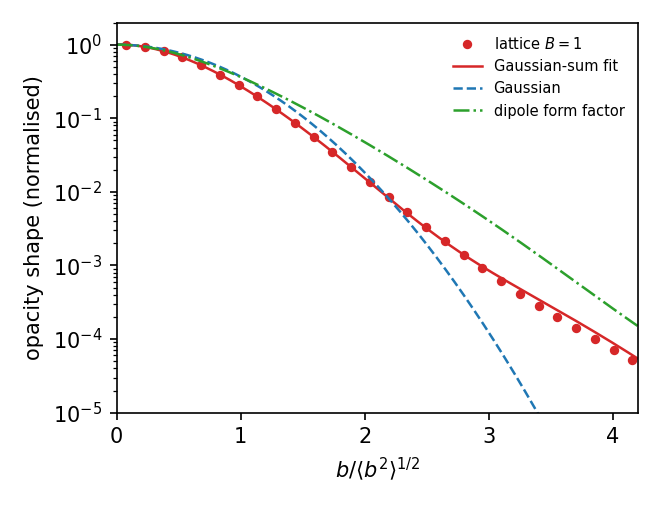
\includegraphics[width=\columnwidth]{../../figures/frame_profile.png}
\caption{Column density of the relaxed $B=1$ frame-sector soliton (points),
its non-negative Gaussian-sum representation (solid), and the two opacity shapes
assumed in Sec.~\ref{sec:scattering}, all normalised to unit rms radius. The
derived profile has a more compact core than either and a tail lying between
them: heavier than a Gaussian beyond $b\simeq2\langle b^2\rangle^{1/2}$, lighter
than the dipole. It is used in Sec.~\ref{sec:scattering} only as a third shape
against which to test robustness.}
\label{fig:frame}
\end{figure}

What the frame sector does \emph{not} establish is a quantitative model of the
proton, and we want to be blunt about this because the temptation to claim it is
obvious. The massless Skyrme model has no pion mass, so its tails are power laws
where the physical ones are exponential; the solitons are unquantised classical
fields, with no spin-isospin projection, no vector mesons and no Casimir
corrections. Its $B=1$ energy is a $30\%$ overestimate of the nucleon mass in the
standard calibration~\cite{adkins1983}. We therefore do \emph{not} use the frame
sector to derive proton structure. Its profile enters Sec.~\ref{sec:scattering}
in one limited role: as a third opacity shape, physically motivated and with a
tail intermediate between the Gaussian and the dipole, against which the
robustness of the forward conclusions can be tested.

\section{Spin-statistics from topology}
\label{sec:spin}

Classical fields normally quantise as bosons, and this was the strongest
objection to soliton models of fermions until Finkelstein and
Rubinstein~\cite{finkelstein1968} showed that the statistics of a soliton is
fixed by the topology of its configuration space $\mathcal{C}_Q$ rather than by
the field's tensor character. A $2\pi$ rotation of a localised configuration
traces a loop $\gamma_{2\pi}$ in $\mathcal{C}_Q$; if $[\gamma_{2\pi}]$ is a
non-trivial element of $\pi_1(\mathcal{C}_Q)$ of order two, the wavefunctional may
be chosen to change sign, and the soliton is a fermion.

For Hopf solitons this analysis was carried out by Krusch and
Speight~\cite{krusch2006}, who showed that the Finkelstein--Rubinstein
constraints admit fermionic quantisation precisely when $\Qh$ is \emph{odd}.
Hence a $\Qh=\pm1$ defect---the topological ground state---carries half-integer
spin and obeys the exclusion principle, while even-$\Qh$ states quantise as
bosons.

Two points of honesty. First, this is a statement that fermionic quantisation is
\emph{consistent and canonical}, not that it is unique: the choice is fixed by the
presence or absence of a topological term in the action, exactly as for
Skyrmions~\cite{witten1983}. The relevant term here is not the five-dimensional
Wess--Zumino form appropriate to an $S^3$ target: for an $S^2$-valued field in
four dimensions it is the $\mathbb{Z}_2$ term classified by
$\pi_4(S^2)=\mathbb{Z}_2$, the four-dimensional counterpart of the Hopf term of
Wilczek and Zee~\cite{wilczekzee1983}. Second, it explains the spin of the
framework's ground state, not the fermion spectrum; the framework does not yet
possess a generation structure (Sec.~\ref{sec:nogo}).

\section{Dynamics of topological transitions}
\label{sec:dynamics}

\subsection{When can $\Qh$ change?}

$\Qh$ is a homotopy invariant of maps $S^3\to S^2$. A continuous, finite-energy
solution of~\eqref{eq:eom} \emph{is} a homotopy, so $d\Qh/dt=0$. The charge can
change only if the director ceases to be defined somewhere---the order parameter
must melt at a point, leaving the vacuum manifold $S^2$. This makes the
annihilation mechanism explicit:

\begin{quote}
An electron and a positron do not annihilate because their invariants ``cancel
during the collision''. They annihilate because the pair was \emph{never in a
protected sector}: a $\Qh=+1$ and a $\Qh=-1$ defect together have total $\Qh=0$,
and nothing forbids relaxation of a $\Qh=0$ configuration to the vacuum plus
radiation. Topological protection is a statement about the \emph{total} charge of
an isolated system, not about individual constituents.
\end{quote}

\subsection{Numerical experiment}

To exhibit this we evolve~\eqref{eq:eom}---with the standard constrained kinetic
term, terms quartic in time derivatives omitted, valid at the sub-relativistic
approach speed $v=0.3c$ used---for two collisions that differ \emph{only} by a
spatial reflection of one constituent: (a) $\Qh=+1$ meets $\Qh=-1$, total
$\Qh=0$; (b) $\Qh=+1$ meets $\Qh=+1$, total $\Qh=+2$. Both initial
configurations have total energy $1126.2$ and are mirror-symmetric about $z=0$.
An absorbing collar removes outgoing radiation so that localised and radiated
energy can be separated.

\begin{table}[t]
\caption{Collision outcomes ($N=96$, $L=20$, $h=0.208$, $2600$ steps, $v=0.3c$,
core sphere $r<5$). The two runs differ only in total topological charge.}
\label{tab:dynamics}
\begin{ruledtabular}
\begin{tabular}{lcccc}
 & $\Qh$ initial $\to$ final & $E_{\rm core}$ initial $\to$ final & retained & remnant $E$ \\
\colrule
(a) annihilation, $\Qh=0$  & $-0.0000\to+0.0000$ & $984.4\to1.9$   & $0.2\%$  & $22.8$ \\
(b) fusion, $\Qh=+2$       & $+1.9791\to+1.9851$ & $957.1\to881.6$ & $77.2\%$ & $888.8$ \\
\end{tabular}
\end{ruledtabular}
\end{table}

The contrast is complete (Table~\ref{tab:dynamics}). The $\Qh=0$ pair converts
$99.8\%$ of the energy initially localised within the core sphere into outgoing
director radiation, leaving no localised remnant; the $\Qh=2$ pair cannot, and
instead sheds only its binding energy. Both runs conserve the charge to better
than $0.4\%$ over $2600$ time steps, itself a stringent test of the
discretisation.

The sharpest check is the last column. The fusion remnant has static energy
$888.8$, while the $\Qh=2$ soliton obtained by direct energy minimisation
(Table~\ref{tab:spectrum})---an independent calculation, on a different lattice,
from a different initial condition---has $\Ehat_2=884.2$. The two agree to
$0.5\%$: the collision product \emph{is} the $\Qh=2$ soliton, so the framework's
static spectrum and its dynamics are consistent with one another.

\subsection{What the released energy is}

Linearising~\eqref{eq:eom} about $\nv=-\hat z$ with $\nv=(\theta_1,\theta_2,
\ldots)$, the quartic invariant is $O(\theta^4)$ and drops out, leaving
$c_2\,\partial_\mu\partial^\mu\theta_a=0$ for $a=1,2$: exactly two transverse,
massless modes propagating at $c$. At quartic order the same term generates a
four-wave self-interaction; for canonically normalised
$\phi_a=\sqrt{2c_2}\,\theta_a$,
\begin{equation}
\mathcal{L}_4=-\frac{c_4}{4c_2^2}\Big[(\partial\phi_1)^2(\partial\phi_2)^2
-(\partial\phi_1\!\cdot\!\partial\phi_2)^2\Big],
\end{equation}
with coupling $g_4=c_4/4c_2^2=\Ehat R^3/(4\Rhat^3M)$ in natural units. This is
directly comparable with the Euler--Heisenberg four-photon
coupling~\cite{eulerheisenberg1936} $2\alpha^2/45m_e^4$, measured in
ultraperipheral heavy-ion collisions~\cite{atlaslbl2019}. Requiring the induced
light-by-light amplitude to stay below $10\%$ of the QED one gives a derived
consistency bound on the core size of a lepton-scale defect,
\begin{equation}
R<0.79\ \mathrm{fm},
\end{equation}
satisfied by four orders of magnitude given the LEP compositeness limit
$R\lesssim10^{-19}\,$m~\cite{bourilkov2001}; at that radius the framework's
contribution to light-by-light scattering is $2.0\times10^{-13}$ of the QED
value. The framework passes this test rather than merely evading it, and the same
formula predicts a $6.5\times10^{-5}$ relative effect for a proton-scale director
soliton.

\section{Topological selection rules and the Standard Model}
\label{sec:sm}

\subsection{The order-parameter hierarchy}

Take the vacuum's local state to be a spinor frame $q\in SU(2)\cong S^3$; the
director is its Hopf projection $\nv=q\sigma_3q^\dagger\in S^2$. The Hopf
fibration~\cite{hopf1931} $S^1\hookrightarrow S^3\to S^2$ is then not an analogy
but the structure of the order parameter itself. Table~\ref{tab:homotopy} lists
the admissible defects. The $SU(3)$ entries follow from the long exact sequences
of $T^2\to SU(3)\to SU(3)/T^2$ and
$\mathbb{Z}_3\to SU(3)\to SU(3)/\mathbb{Z}_3$ using
$\pi_1(SU(3))=\pi_2(SU(3))=0$, $\pi_3(SU(3))=\mathbb{Z}$.

\begin{table}[t]
\caption{Homotopy content of the candidate order parameters. The $\pi_2$ and
$\pi_3$ columns classify defects proper---point defects and textures
respectively---while a non-trivial $\pi_1$ is realised in three dimensions as a
line defect, and enters below as a selection rule on admissible sources rather
than as an isolated particle.}
\label{tab:homotopy}
\begin{ruledtabular}
\begin{tabular}{lcccl}
order parameter & $\pi_1$ & $\pi_2$ & $\pi_3$ & topological content \\
\colrule
$S^2$ (director)     & $0$ & $\mathbb{Z}$ & $\mathbb{Z}$ & hedgehogs; Hopfions \\
$S^3=SU(2)$ (frame)  & $0$ & $0$ & $\mathbb{Z}$ & Skyrmions~\cite{skyrme1961}, degree $=$ baryon no. \\
$S^1$ (Hopf fibre)   & $\mathbb{Z}$ & $0$ & $0$ & charge quantisation \\
$SU(3)/T^2$ (flag)   & $0$ & $\mathbb{Z}^2$ & $\mathbb{Z}$ & rank-2 colour lattice \\
$SU(3)/\mathbb{Z}_3$ & $\mathbb{Z}_3$ & $0$ & $\mathbb{Z}$ & triality classes \\
\end{tabular}
\end{ruledtabular}
\end{table}

\subsection{Charge quantisation from the fibre}

The director determines the frame only up to the $U(1)$ fibre phase, whose
winding around a closed loop lies in $\pi_1(S^1)=\mathbb{Z}$. Identifying it with
electric charge gives exact quantisation with no magnetic monopole required---the
Dirac argument is replaced by the fibration itself. The Hopf invariant is the
linking number of the preimages of any two distinct regular values, so charge and
$\Qh$ are two readings of the same fibration, which is why they are correlated in
the ground state.

\subsection{Colour and confinement as a selection rule}

For an $SU(3)$-valued frame the Cartan torus gives
$\pi_2(SU(3)/T^2)=\mathbb{Z}^2$: a rank-two charge lattice, i.e.\ the weight
lattice, whose fundamental representation has three weights summing to
zero---three colours, permuted by the Weyl group $S_3$. The centre gives
$\pi_1(SU(3)/\mathbb{Z}_3)=\mathbb{Z}_3$: triality.

A source carrying non-zero triality cannot be screened by the adjoint content of
the vacuum, since screening would require a continuous deformation between
distinct classes of $\pi_1(SU(3)/\mathbb{Z}_3)$. In three dimensions such a class
is carried by a line defect, so the flux joining triality sources is a tube
rather than a Coulomb field---the picture of 't~Hooft's centre
vortices~\cite{thooft1978}---and it must terminate on a triality-compensating
source. No isolated finite-energy configuration of non-zero triality exists, and
only triality-neutral combinations---$qqq$, $\bar q\bar q\bar q$, $q\bar q$---are
admissible.

We should be clear about the standing of this observation. It is a statement
about what the topology permits, not a dynamical account of confinement: the
centre classes forbid isolated triality but say nothing about the string tension,
the spectrum, or the approach to the continuum, all of which are properties of
the quantum gauge theory rather than of a classical order parameter. Nor is it
joined to the computations of this paper, which are $S^2$ and $SU(2)$ throughout.
We record it as a geometric analogy that the framework makes available, and note
that it is the same $\mathbb{Z}_3$ that makes baryon number per quark equal to
$1/3$: fractional winding cannot be isolated for the identical reason.

This is the point of contact with established results. Faddeev and
Niemi~\cite{faddeev1997,faddeev1999}, building on Cho's
decomposition~\cite{cho1980}, argue that the infrared effective theory of $SU(2)$
Yang--Mills is the Faddeev--Skyrme model of exactly the director field used here,
with knotted solitons as glueball candidates. The elastic derivation of
Sec.~\ref{sec:elastic} is thus not in competition with QCD; it supplies a
continuum-mechanical reading of a decomposition already used in gauge theory.

\subsection{Neutral leptons}

A lepton in this classification carries two independent labels: the Hopf
invariant (self-linking of the fibres) and the net fibre winding (charge). A
defect with $\Qh=\pm1$ and \emph{zero} net fibre winding is a neutral lepton: it
is topologically a lepton, has no long-range field, and---because the
electromagnetic self-energy contribution to its mass vanishes identically---its
mass is not bounded below by that contribution and can be parametrically small.
This accounts qualitatively for the existence and lightness of neutrinos. It is
not a mass prediction and we do not present it as one.

\section{What the director sector cannot contain}
\label{sec:nogo}

Stated plainly:

\emph{Generations---and a no-go.} The $|\Qh|=1$ sector has a unique ground state,
so there is no topological label distinguishing $e,\mu,\tau$. We can sharpen
this. By~\eqref{eq:shape}, at fixed couplings the mass ratio of two states is the
ratio of their shape constants, and $\Ehat$ grows only as $|\Qh|^{3/4}$.
Reproducing $m_\mu/m_e=206.77$ would require $|\Qh|\simeq1.2\times10^3$, and
$m_\tau/m_e=3477$ would require $|\Qh|\simeq5\times10^4$---with, by
Sec.~\ref{sec:spin}, both charges odd.

The obvious escape is that the extra states are not new topological sectors but
excitations of the same one: a soliton has a spectrum of internal oscillations,
and those carry the same charge and the same spin at higher mass, which is
exactly what a generation looks like. That escape is closed, and it is worth
closing quantitatively rather than by assertion, because the homotopy argument
above says nothing about it.

The director is massless---its vacuum manifold is $S^2$, so fluctuations about
the vacuum are Goldstone modes---so the radiation continuum reaches down to zero
frequency and any internal oscillation is embedded in it. Whether it is
nonetheless long lived is a matter of measurement. Exciting the breathing mode of
the $\Qh=1$ soliton by a $6\%$ dilation and evolving with an absorbing collar,
the energy radius rings and decays:
\begin{equation}
\omega = 0.486, \qquad \Gamma = 0.059, \qquad \Gamma/\omega = 0.12 .
\label{eq:breather}
\end{equation}
The mode is real---it completes about five periods---but it is a resonance of
hadronic width, comparable to the $\Delta$ at $\Gamma/m\simeq0.12$. A muon
requires $\Gamma/m\simeq3\times10^{-18}$. Vibrational quantisation therefore
misses by some sixteen orders of magnitude, and since numerical dissipation can
only inflate the measured width, Eq.~\eqref{eq:breather} is an upper bound on how
narrow such a state could be.

A second escape survives that argument. Besides vibrations a soliton has
\emph{zero} modes, and rigid-body quantisation of those also produces a tower at
fixed charge and fixed spin; zero modes do not decay, so the width bound does not
touch them. This route closes quantitatively too. For a collective coordinate
$\nv\to e^{\theta K}\nv$ the kinetic term $c_2|\partial_t\nv|^2$ gives
$T=\tfrac12\Lambda\dot\theta^2$ with $\Lambda=2c_2\!\int\!|K\nv|^2$ and a tower
$E_k=k^2/2\Lambda$. Measured on the relaxed $\Qh=1$ field, the internal $U(1)$
that rotates the target about the vacuum axis and the spatial rotations give
\begin{equation}
\Lambda_{U(1)}=217.7,\quad \Lambda_{\perp}=281.5,\quad \Lambda_{\parallel}=232.8,
\qquad \frac{1}{2\Lambda_{U(1)}M_1}=4.2\times10^{-6},
\label{eq:collective}
\end{equation}
the two transverse moments agreeing to five digits as the axial symmetry of the
$\Qh=1$ solution requires. The level spacing is four parts in $10^{6}$ of the
soliton mass: the tower is near-degenerate, not a generation ladder. Reaching
$m_\mu/m_e$ would need $k\simeq7.0\times10^{3}$, at which the collective
frequency $k/\Lambda=32$ exceeds the soliton's own breathing frequency $0.486$
by a factor of $66$---the adiabatic separation that justified treating the body
as rigid has failed by two orders of magnitude---and the state would in any case
lie some $200$ times its own mass above the one-soliton threshold. Quartic
contributions to $\Lambda$ are positive definite, so including them only lowers
the spacing and raises the required $k$: the exclusion is conservative.

What remains is to enlarge the target manifold so that the $|\Qh|=1$ sector
carries an additional discrete label. We do not claim that no such enlargement
exists---that is the principal open problem---but its price can be stated
exactly, and within this framework it is high. Let $X$ be the enlarged target,
required to keep $\pi_3(X)=\mathbb{Z}$ so that the charge-one state remains
protected. Three costs follow.

\emph{(i) Theorem~1 does not survive.} By the corollary of
Sec.~\ref{sec:corollary}, $I_k\equiv0$ only for $k>\min(\dim X,3)$. Any $X$ with
$\dim X\ge3$ therefore admits $I_3\not\equiv0$, a sextic invariant becomes
writable, and the Mooney--Rivlin form stops being an exact truncation and becomes
a choice carrying a third independent elastic constant. This is measured, not
hypothetical: the frame sector, with $\dim S^3=3$, already gives
$|\det D|/I_1^3=3.7\times10^{-2}$ against $10^{-7}$ for the director. The one
property that made the quartic term non-optional is lost on any enlargement.

\emph{(ii) Degeneracy, or the wrong quantum numbers.} If the candidate states are
related by a symmetry of the energy they are exactly degenerate and must be split
by an explicit breaking term. The natural candidate has this form: in the flag
manifold $SU(3)/T^2$---which does keep $\pi_3=\mathbb{Z}$, since
$\pi_3(T^2)=0\to\pi_3(SU(3))=\mathbb{Z}\to\pi_3(SU(3)/T^2)\to\pi_2(T^2)=0$---the
three $SU(2)$ subgroups are conjugate, their Weyl images forming a single class,
so the three embedded solitons have rigorously equal energy. If instead the
states are not related by a symmetry, they will generically differ in spin or in
charge, whereas generations are copies differing only in mass.

\emph{(iii) The parameter count inverts.} Splitting a degenerate triplet requires
at least two independent couplings, which together with the revived sextic
constant makes three new parameters accommodating the two ratios $m_\mu/m_e$ and
$m_\tau/m_e$. A construction with more free parameters than observables is a fit,
not a prediction, and it would forfeit exactly the restraint that makes
Theorem~2 a matching identity rather than a claim to have explained the
hierarchy.

One route can be excluded outright rather than priced. A label carried by
$\pi_2(X)$---for instance the second factor of
$\pi_2(SU(3)/T^2)=\mathbb{Z}\oplus\mathbb{Z}$---does not describe a lepton: a
configuration with nonzero $\pi_2$ charge is a hedgehog whose energy grows
linearly with the box and whose field falls off as $r^{-2}$. This is not a new
hazard introduced by enlargement, since $\pi_2(S^2)=\mathbb{Z}$ and the director
sector already contains such defects; in both cases they are excluded because
they are singular, and in both cases they are point defects rather than internal
labels of a localised soliton.

The standing of this subsection is therefore stronger than an admission of
ignorance and weaker than a proof of impossibility. Generations do not arise
from new topological sectors, from vibrational excitation, or from collective
quantisation, and every route out of the director sector that we can identify
costs more parameters than it explains. The $S^2$ hyperelastic medium appears to
have no room for them.

\emph{Mass ratios and Yukawa couplings.} Not addressed.

\emph{CP violation, the CKM matrix, and the Cabibbo angle.} Not addressed.

\emph{Quantisation of the metric sector.} We treat the metric classically and the
director sector semiclassically. How the continuum survives quantisation is open.

\section{Forward elastic $pp$ scattering: a constraint}
\label{sec:scattering}

This section is deliberately self-contained and is the one part of the paper that
is phenomenological rather than derived. It asks a single question---does the
finite rigidity established in Sec.~\ref{sec:elastic} leave an observable trace
in forward hadronic scattering?---and answers it as an observational bound on one
parameter. A reader interested only in the geometric and computational results
may stop at Sec.~\ref{sec:sm} without loss; nothing earlier depends on what
follows.

\subsection{The prediction}

The Froissart--Martin bound~\cite{froissart1961,martin1963} permits
$\sigma_{\rm tot}\le(\pi/\mu^2)\ln^2(s/s_0)$, and conventional eikonal models
saturate it. The bound itself is numerically very weak---of order
$5\times10^3\,$mb at $13\,$TeV---so ``bounding the Froissart limit'' is not a
meaningful prediction. The meaningful statement is different and stronger:

\begin{quote}
A medium of finite rigidity cannot transmit unbounded strain, so the
\emph{interaction radius} of an extended soliton must itself saturate. The
asymptotic growth of $\sigma_{\rm tot}$ is then $\ln s$, not $\ln^2 s$, and
because analyticity ties $\rho$ to the local logarithmic growth rate,
$\rho\simeq\tfrac{\pi}{2}\,d\ln\sigma_{\rm tot}/d\ln s$, the asymptotic $\rho$ is
halved.
\end{quote}

We implement this minimally. With $L=\ln(s/s_0)$ and a Pomeron-like opacity
$\Omega(b,s)=Ce^{\Delta L}\exp(-b^2/R^2)$, the conventional model has
$R^2_{\rm bare}=R_0^2+4\alpha' L$; the framework replaces
\begin{equation}
R\longrightarrow R_\infty\tanh\!\big(R_{\rm bare}/R_\infty\big),
\end{equation}
which is \emph{nested}: $R_\infty\to\infty$ recovers the conventional model
exactly, so the two hypotheses can be compared by a likelihood ratio with one
extra parameter. Crossing-even analyticity supplies the real part with no
additional freedom through $L\to\ln(s/s_0)-i\pi/2$; $\rho$ is a prediction, not a
fit parameter.

The $\tanh$ is a minimal phenomenological implementation. The framework's content
is that a bound exists and is set by the medium's rigidity, not the functional
form by which it is approached. That distinction is testable rather than
rhetorical, and we have tested it. Repeating the fit and the profile likelihood
with $R_\infty(1-e^{-R_{\rm bare}/R_\infty})$ and with the algebraic
$R_{\rm bare}(1+R_{\rm bare}^2/R_\infty^2)^{-1/2}$---three forms sharing the same
two limits but approaching the bound at very different rates, exponentially in
two cases and as a power in the third---moves the best fit from $\chi^2=39.74$ to
$39.81$ and $39.79$, against $40.78$ unsaturated, and moves the predicted
$\rho(13\,\mathrm{TeV})$ from $0.1144$ to $0.1146$. The $95\%$ lower limit is
$1.18\,$fm in all three cases, unchanged to the $0.1\,$fm resolution of the scan,
even though the best-fit $R_\infty$ itself ranges over $1.30$ to $1.45\,$fm as
the saturation rate changes. The limit is therefore a property of the data and
not of the parameterisation. What does move it is the assumed opacity profile
(Sec.~\ref{sec:profile}), which is why we quote the conservative
$\gtrsim1.0\,$fm rather than $1.18\,$fm.

What the framework does require is that
$R_\infty$ be of order the soliton's own extent, since the bound arises from the
soliton's finite stored strain and not from a new scale. The fit returns
$R_\infty=6.59\,\mathrm{GeV}^{-1}=1.30\,$fm against a proton interaction radius
of $\simeq1.0\,$fm at LHC energies, which is the required consistency.

\subsection{Fit to world data}

Fitting $\sigma_{\rm tot}$, $\rho$ and the forward slope $B$ from UA4/2, E710,
TOTEM and ATLAS-ALFA ($546\,$GeV to $13\,$TeV; 22
measurements)~\cite{ua42,e710,totem2020,atlas2014,totem2016,atlas2016,totem2019rho,atlas2023}
gives $\chi^2=40.78/18$ dof for the conventional model and $39.74/17$ dof for the
rigidity-saturated one. Thus $\Delta\chi^2=1.03$ for one extra parameter:
\emph{current data do not discriminate}, which we state as the result rather than
claiming a preference. The $\chi^2/$dof of $\sim2.3$ is dominated by known
experimental tensions---chiefly the $2.5\sigma$ TOTEM/ATLAS disagreement on
$\sigma_{\rm tot}(13\,\mathrm{TeV})$---not by the model.

The profile likelihood over $R_\infty$, with all other parameters re-minimised,
is sharply one-sided and yields $R_\infty>1.14\,$fm at $95\%$ CL with the
Gaussian profile. This moves by $-0.15$ to $+0.24\,$fm depending on the assumed
impact-parameter shape (Sec.~\ref{sec:profile}), so we quote
\begin{equation}
\boxed{\;R_\infty \gtrsim 1.0\ \mathrm{fm}\ \ (95\%\ \mathrm{CL}).\;}
\end{equation}
The scan grid limits the precision of any single such limit to about
$0.05\,$fm, which is well below the profile and dataset systematics quoted
below.
Repeating on subsets (Table~\ref{tab:systematics}) shows the bound is stable at
$1.0$--$1.2\,$fm and is not an artefact of the TOTEM/ATLAS disagreement. That the
ATLAS-only fit has $\chi^2/$dof $=1.18$ while the combined fit has $2.27$
confirms the poor combined $\chi^2$ is experimental.

\begin{table}[t]
\caption{Dependence of the fit and the rigidity bound on the data subset.}
\label{tab:systematics}
\begin{ruledtabular}
\begin{tabular}{lccccc}
dataset & $N$ & $\chi^2/$dof (conv.) & $\chi^2/$dof (sat.) & $\Delta\chi^2$ & $R_\infty$ limit \\
\colrule
all                   & 22 & 2.27 & 2.34 & 1.03 & $1.14\,$fm \\
TOTEM only at LHC     & 16 & 2.16 & 2.31 & 0.43 & $1.04\,$fm \\
ATLAS-ALFA only       & 13 & 1.18 & 1.33 & 0.01 & $1.14\,$fm \\
LHC $pp$ only         & 15 & 2.51 & 2.68 & 0.72 & $1.18\,$fm \\
\end{tabular}
\end{ruledtabular}
\end{table}

\begin{figure}[t]
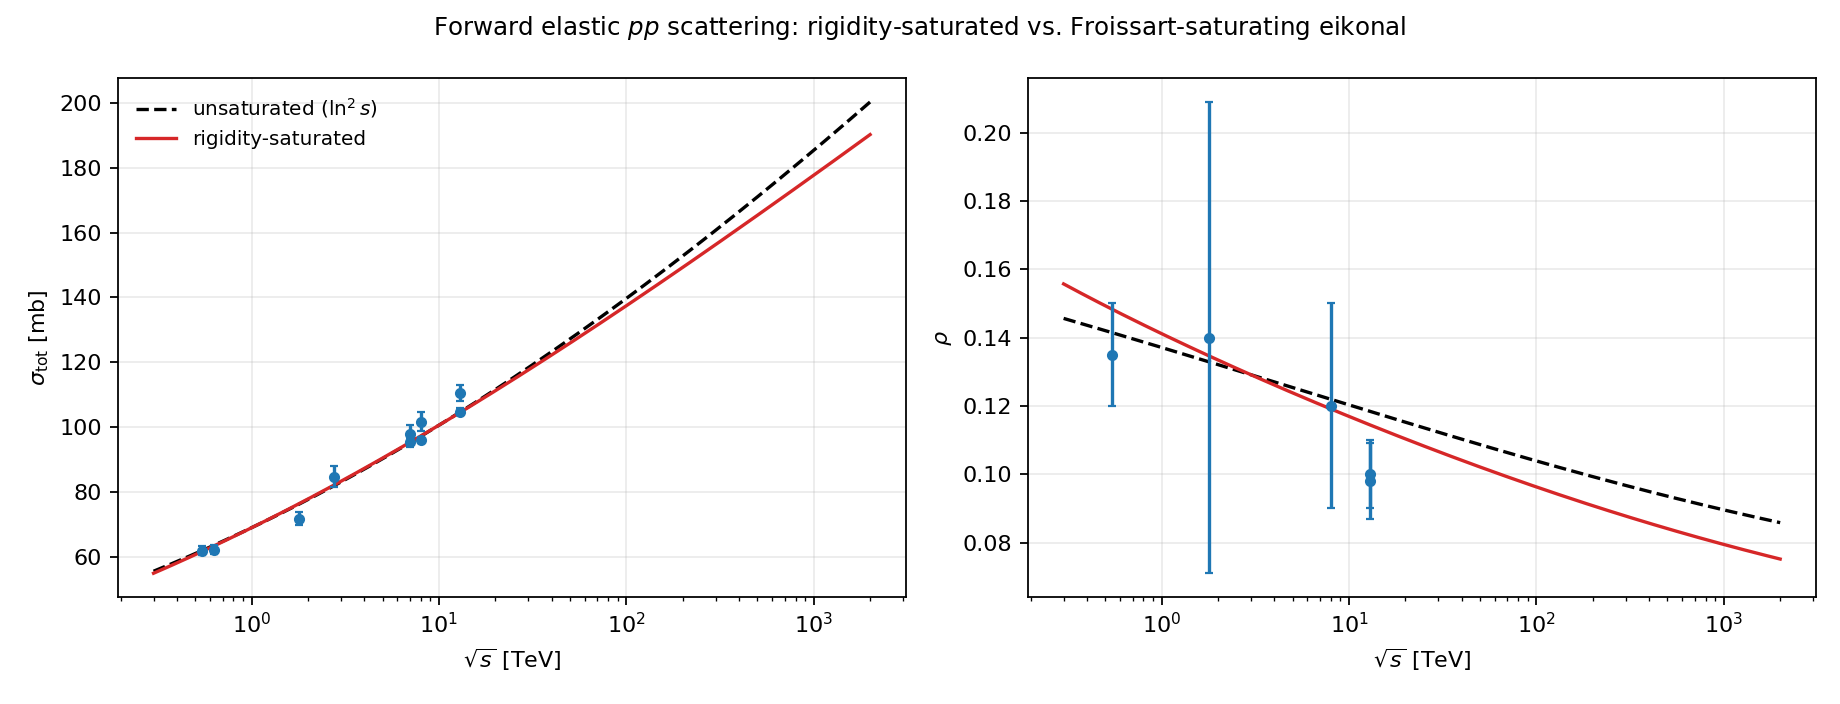
\includegraphics[width=\columnwidth]{../../figures/forward_scattering.png}
\caption{Forward elastic $pp$ scattering. Dashed: conventional
Froissart-saturating eikonal. Solid: rigidity-saturated. Points: measurements
used in the fit.}
\label{fig:forward}
\end{figure}

\subsection{Predictions and falsification criteria}

\begin{table}[t]
\caption{Predictions of the two nested hypotheses (conventional / saturated).}
\label{tab:predictions}
\begin{ruledtabular}
\begin{tabular}{lcccc}
$\sqrt{s}$ & $\sigma_{\rm tot}$ (mb) & $\rho$ & $B$ (GeV$^{-2}$) & $\sigma_{\rm el}/\sigma_{\rm tot}$ \\
\colrule
$7\,$TeV   & 95.2 / 95.3   & 0.1229 / 0.1204 & 19.5 / 19.5 & 0.272 \\
$8\,$TeV   & 97.2 / 97.2   & 0.1219 / 0.1191 & 19.7 / 19.8 & 0.275 \\
$13\,$TeV  & 104.7 / 104.5 & 0.1184 / 0.1144 & 20.8 / 20.8 & 0.284 \\
$14\,$TeV  & 105.8 / 105.7 & 0.1178 / 0.1137 & 21.0 / 21.0 & 0.286 \\
$27\,$TeV  & 116.6 / 115.9 & 0.1131 / 0.1076 & 22.7 / 22.5 & 0.298 \\
$100\,$TeV & 139.7 / 137.4 & 0.1039 / 0.0963 & 27.0 / 26.4 & 0.321 \\
\end{tabular}
\end{ruledtabular}
\end{table}

From Table~\ref{tab:predictions}:

\begin{enumerate}
\item $\rho$ is the discriminating observable, not $\sigma_{\rm tot}$. At
$100\,$TeV the two hypotheses differ by $1.6\%$ in $\sigma_{\rm tot}$ but $8\%$
in $\rho$; a measurement of $\rho(100\,\mathrm{TeV})$ to $\pm0.004$ separates
them at $2\sigma$.
\item If $\sigma_{\rm tot}$ is measured to grow faster than $\ln^2 s$ at any
energy, the rigidity bound is excluded outright.
\item If $\sigma_{\rm el}/\sigma_{\rm tot}$ exceeds $1/2$ at any energy, the
eikonal-with-finite-radius picture fails.
\item The framework accommodates without an Odderon what TOTEM identified as the
alternative reading of its $13\,$TeV measurement: if three-gluon exchange is not
responsible, the measured $\rho$ ``would represent a first evidence of a slowing
down of the total cross-section growth at higher
energies''~\cite{totem2019rho}. A slowing of the growth is exactly what finite
vacuum rigidity requires. In the interest of not overstating this, the present
crossing-even fit still returns $\rho(13\,\mathrm{TeV})=0.114$ against the
measured $0.098\pm0.011$---a $1.4\sigma$ tension in the direction the model needs
but does not yet fully deliver.
\end{enumerate}

\subsection{Profile dependence and the diffractive dip}
\label{sec:profile}

A Gaussian opacity profile is a convenience, and it is fair to ask whether the
conclusions are an artefact of it. We therefore repeated the entire analysis with
two further shapes. The first is the profile implied by the \emph{measured}
proton dipole form factor, $G(t)=(1+|t|/\Lambda^2)^{-2}$, whose overlap function
is proportional to $u^3K_3(u)$ with $u=\Lambda b$. The second is
\emph{computed}: the column density of the relaxed $B=1$ frame-sector soliton of
Sec.~\ref{sec:frame} (Fig.~\ref{fig:frame}), which is not fitted to scattering
data at all. To keep the crossing-even continuation available with a non-Gaussian
shape, each profile is represented as a sum of Gaussians with non-negative
amplitudes on a fixed logarithmic width grid---every term remains analytic in
$R^2$---reproducing $u^3K_3(u)$ to an rms residual of $2\times10^{-8}$ with
eleven terms, and the lattice column density to $1\times10^{-4}$ with six.

The three shapes are genuinely different: at equal rms radius the computed
profile has the most compact core, and a tail heavier than the Gaussian beyond
$b\simeq2\langle b^2\rangle^{1/2}$ but lighter than the dipole. The outcome is
twofold.

\emph{The forward conclusions are insensitive to the profile.} The fit quality is
essentially unchanged ($\chi^2=40.7$ and $40.6$ against $39.7$ for the Gaussian),
as are all the forward observables:
$\rho(13\,\mathrm{TeV})=0.1144,\,0.1151,\,0.1150$ for Gaussian, dipole and
computed profiles, with
$\sigma_{\rm tot}(13\,\mathrm{TeV})=104.5\,$mb and
$B(13\,\mathrm{TeV})=20.8\,$GeV$^{-2}$ in all three. The rigidity bound is
$R_\infty>1.14,\,0.99,\,1.38\,$fm respectively, so together with
the dataset systematics of Table~\ref{tab:systematics} the honest statement is
\begin{equation}
R_\infty \gtrsim 1.0\ \mathrm{fm}\quad (95\%\ \mathrm{CL}),
\end{equation}
with profile and dataset systematics spanning $0.99$--$1.38\,$fm. The bound is
set by the least constraining shape, which is the dipole.

\emph{The dip is reproduced once the profile is realistic.} The Gaussian places
the first diffractive minimum at $|t_{\rm dip}|=1.29\,$GeV$^2$ at $7\,$TeV
against the measured $0.53\,$GeV$^2$, and generates a spurious second minimum;
its tail simply falls too fast. The dipole profile gives a single clean minimum
at $0.494\,$GeV$^2$, within $7\%$ of the measurement, and reproduces the observed
energy dependence:

\begin{table}[t]
\caption{Diffractive minimum $|t_{\rm dip}|$ in GeV$^2$, for the dipole and the
computed frame-sector profiles (rigidity-saturated fit). The two growth
hypotheses are indistinguishable here---they differ by under $1\%$ even at
$100\,$TeV---so the dip validates the eikonal but does not discriminate;
$\rho$ remains the only discriminating observable.}
\label{tab:dip}
\begin{ruledtabular}
\begin{tabular}{cccc}
$\sqrt{s}$ & dipole & computed & measured \\
\colrule
$2.76\,$TeV & 0.594 & 0.508 & 0.72 \\
$7\,$TeV    & 0.493 & 0.436 & 0.53 \\
$8\,$TeV    & 0.481 & 0.426 & 0.52 \\
$13\,$TeV   & 0.440 & 0.396 & 0.47 \\
$14\,$TeV   & 0.435 & 0.391 & --- \\
$27\,$TeV   & 0.388 & 0.355 & --- \\
$100\,$TeV  & 0.315 & 0.297 & --- \\
\end{tabular}
\end{ruledtabular}
\end{table}

The dipole runs $7$--$18\%$ below the measured positions but tracks the energy
dependence correctly, which is a non-trivial check on the eikonal at momentum
transfers an order of magnitude beyond those it was fitted to. The computed
profile does noticeably worse, $18$--$29\%$ low, and we report that plainly: it
is the one place where deriving the shape rather than measuring it costs
accuracy, and it is the expected direction, since a massless Skyrme soliton has
power-law rather than pion-range tails and the dip is controlled by exactly that
part of the profile.

We note for completeness that the proton is not a Hopfion in this framework but a
baryon-number defect of the frame sector, $\pi_3(SU(2))$, which is why the
computed profile above is taken from Sec.~\ref{sec:frame} and not from the
director solitons of Sec.~\ref{sec:spectrum}. It is used as a third shape and
nothing more; we are not proposing the massless Skyrme soliton as a model of
proton structure, for the reasons set out in Sec.~\ref{sec:frame}.

\subsection{Status of this sector}

We state the outcome plainly rather than as a claimed success. The
rigidity-saturated hypothesis fits the world data no better and no worse than the
conventional one; the data bound $R_\infty$ from below but do not favour a finite
value; and the model does not reproduce the $\rho$ anomaly that motivates it,
falling $1.4\sigma$ short in the right direction. What this section establishes
is a \emph{constraint} on the vacuum's rigidity scale, robust against the profile
and dataset choices, together with a sharp statement of which future measurement
would settle the question. It is not evidence for the framework, and we do not
present it as such.

\section{Summary of falsifiable content}
\label{sec:predictions}

A framework of this kind should be judged on what could kill it. We therefore
collect, in one place, every statement the framework commits to, with the
observation that would refute each (Table~\ref{tab:falsify}). We also state
plainly what it does \emph{not} predict, since a list of successes with the
failures omitted is not an honest accounting.

\begin{table*}[t]
\caption{Falsifiable content. Quantitative entries are quoted for the
rigidity-saturated hypothesis against the conventional one where the two differ.}
\label{tab:falsify}
\begin{ruledtabular}
\begin{tabular}{p{0.40\textwidth}cp{0.40\textwidth}}
statement & where & \raggedright refuted by \tabularnewline
\colrule
\raggedright $\sigma_{\rm tot}$ grows asymptotically as $\ln s$, not $\ln^2 s$;
$d\sigma_{\rm tot}/d\ln s\to$ const $\simeq9\,$mb per e-fold
 & \ref{sec:scattering} & \raggedright a growth rate that keeps increasing with
   energy \tabularnewline
\raggedright $\rho(100\,\mathrm{TeV})=0.096$ against $0.104$ conventional
 & \ref{sec:scattering} & \raggedright $\rho$ measured to $\pm0.004$ favouring
   the conventional value \tabularnewline
\raggedright $\sigma_{\rm el}/\sigma_{\rm tot}<1/2$ at every energy
 & \ref{sec:scattering} & \raggedright the ratio exceeding $1/2$ \tabularnewline
\raggedright the rigidity radius is finite, $R_\infty\gtrsim1.0\,$fm
 & \ref{sec:scattering} & \raggedright no slowing of $\sigma_{\rm tot}$ growth at
   any energy \tabularnewline
\raggedright light-by-light amplitude receives a positive addition $\propto R^3$;
$6.5\times10^{-5}$ of QED for a proton-scale core
 & \ref{sec:dynamics} & \raggedright a measured deficit, or an excess of the
   wrong sign \tabularnewline
\raggedright exactly two massless transverse director modes
 & \ref{sec:dynamics} & \raggedright a scalar or longitudinal polarisation in the
   same sector \tabularnewline
\raggedright odd $\Qh$ quantises as a fermion, even $\Qh$ as a boson
 & \ref{sec:spin} & \raggedright an even-charge fermionic soliton \tabularnewline
\raggedright $E_Q<Q\,E_1$: multi-charge defects do not fission
 & \ref{sec:spectrum} & \raggedright an observed fission of a $|Q|>1$ state
   \tabularnewline
\raggedright no isolated configuration of non-zero triality
 & \ref{sec:sm} & \raggedright a free quark \tabularnewline
\raggedright charge is quantised by the integer winding of the Hopf fibre
 & \ref{sec:sm} & \raggedright non-integer charge, or a magnetic monopole in this
   sector \tabularnewline
\raggedright generations cannot arise in the director sector alone
 & \ref{sec:nogo} & \raggedright an $S^2$ director model producing three
   generations \tabularnewline
\raggedright the soliton's internal oscillation is a resonance of hadronic
width, $\Gamma/\omega=0.12$
 & \ref{sec:nogo} & \raggedright a narrow vibrational state in a gapless
   director medium \tabularnewline
\raggedright topological protection requires rigidity at the cutoff
 & \ref{sec:lattice} & \raggedright a protected topological code in a medium with
   a soft cutoff-scale mode \tabularnewline
\end{tabular}
\end{ruledtabular}
\end{table*}

\subsection{What the framework does not predict}

It does not predict particle masses, mass ratios, the fine-structure constant,
the CKM matrix, CP violation, or any new resonance, and it says nothing about
dark matter or dark energy. The no-go of Sec.~\ref{sec:nogo} makes the first two
of these structural rather than merely unfinished: mass ratios cannot come from
the director sector at all.

\subsection{An honest weighting}

Not all of the entries in Table~\ref{tab:falsify} carry the same evidential
weight, and we do not wish to imply otherwise.

Several are \emph{postdictions}: charge quantisation, confinement, and the
$\Qh\le4$ spectrum reproduce facts already known, however satisfying it is to
obtain them from topology rather than to assume them. Their value is as
validation of the machinery, not as evidence for the framework.

The quantitative entries are honest predictions but weak discriminators: the
forward-scattering split is a few parts per thousand in an observable that is
difficult to measure, and it will not be settled below $100\,$TeV. The
light-by-light entry is a genuine prediction with a sharp $R^3$ scaling, but is
numerically tiny for any core size compatible with existing compositeness limits.

The two entries we would point to as most distinctive are the no-go, which
constrains any future extension of the framework rather than the framework
itself, and the requirement of rigidity at the cutoff---which is the only item in
the table that emerged \emph{from} the computation rather than being sought,
and which applies to any physical realisation of a topological code, not only to
the vacuum.

\section{Conclusion}

The framework presented here rests on one theorem, one identity and a
computation. Theorem 1 shows that the Faddeev--Skyrme energy is not a model
choice but the exact isotropic hyperelastic energy of a director field in a
three-dimensional medium, and that the truncation is exact rather than
approximate because the target is two-dimensional. It leaves the medium with
exactly one length, the Cosserat length $\lc$, and no adjustable structure. The
anchoring identity of Sec.~\ref{sec:anchoring} then converts the ratio of
director stiffness to metric tension into the gravitational compactness of the
defect it supports; it restates the Planck-to-particle hierarchy as the
observation that particles are not black holes, and we are careful to claim the
restatement and nothing more.

The lattice computation then does five things the framework previously only
asserted. It reproduces the published $\Qh\le4$ Faddeev--Skyrme spectrum to
$0.6$--$1.6\%$, together with all four ground-state configuration types, from
independent seeds and a different discretisation---and, once extrapolated to zero
spacing and infinite volume, it disagrees with the published charge-one energy by
$2.2\%$, which we report as an open discrepancy on the strength of the frame
sector validating the extrapolation to $0.03\%$. It finds every
multi-charge sector bound against fission, with $E\propto|\Qh|^{0.765}$
reproducing the Vakulenko--Kapitanskii exponent to $2\%$. It identifies the
$\Qh=4$ ground state as a \emph{linked} configuration lying below the axially
symmetric one. It gives annihilation an explicit dynamical account, with the
$\Qh=0$ pair radiating $99.8\%$ of its localised energy while its mirror image at
$\Qh=+2$ cannot, and with the surviving remnant matching the independently
minimised $\Qh=2$ soliton to $0.5\%$. And it shows that topological protection
fails outright in a medium that is not rigid at its cutoff.

That the dimension count of Theorem 1 is a count, and not a feature of the
director in particular, is what makes it testable in a second place. Carried over
to the frame $S^3$---the only other target a three-dimensional medium admits
without further structure---it predicts that the truncation should fail there,
and it does: a sextic invariant becomes admissible, and it is precisely the term
the Skyrme literature adds by hand. Running the same code in that sector recovers
the exact $B=1$ energy to $0.03\%$ and the published $B=2$ binding to $0.06$
percentage points, so the agreement in Sec.~\ref{sec:spectrum} is not an artefact
of one tuned discretisation.

What the framework does not do is equally important: it has no generation
structure, no mass ratios, and no flavour physics, and Sec.~\ref{sec:nogo}
excludes the routes by which generations might have been recovered---new
topological sectors, vibrational excitation and collective quantisation---and
prices the remaining one, enlargement of the target, at more free parameters
than it would explain.

What remains is falsifiable. The rigidity scale is already bounded from below,
$R_\infty\gtrsim1.0\,$fm at $95\%$ CL, by forward elastic scattering; the framework
predicts $\ln s$ rather than $\ln^2 s$ asymptotic growth of $\sigma_{\rm tot}$
and a correspondingly halved $\rho$, the discriminating measurement being $\rho$
at the highest available energy; and it predicts a calculable, positive addition
to light-by-light scattering scaling as the cube of the soliton core radius.
These are the tests we would ask experimentalists to make.

\begin{acknowledgments}
Numerical work was carried out with NumPy, SciPy, SymPy and Matplotlib. The
author used an AI assistant (GitHub Copilot) for code development, numerical
analysis and manuscript preparation; all physical claims, and responsibility for
them, are the author's.
\end{acknowledgments}

\appendix

\section{Numerical methods}

The lattice construction, its two symmetrised schemes, the minimiser and the
extrapolation procedure are described in the companion paper~\cite{lattice}, and
the source is available at~\cite{repo}. Two items specific to the computations
reported here are recorded below.

\emph{Evolution.} Leapfrog with renormalisation of $|\nv|$, the constraint term
$-|\dot{\nv}|^2\nv$, and an absorbing collar. Terms quartic in time derivatives
are omitted; this is controlled at the collision speeds used and is stated as an
approximation, not a result.

\emph{Frame sector.} The energy, its gradient, the normalisation, the Derrick
rescaling and the minimiser are all written in terms of the number of target
components and are used unaltered for $S^3$; only the charge estimator differs,
Eq.~\eqref{eq:baryon} being evaluated as the determinant of the
$4\times4$ matrix $[\varphi,\partial_1\varphi,\partial_2\varphi,\partial_3\varphi]$
at every site.

\section{Reproducibility}

The computational supplement~\cite{repo} comprises a library (\texttt{rt/}) and
drivers (\texttt{scripts/}), shared with~\cite{lattice}. The library modules are
\texttt{constants.py}
(CODATA-2018 constants, $\Gamma$); \texttt{invariants.py} (symbolic verification
of Theorem 1 and the virial identity); \texttt{fs\_core.py} (lattice energy,
exact gradient, Hopf charge); \texttt{ansatz.py} (seeds of prescribed charge);
\texttt{relax.py} (minimiser, Derrick rescaling, evolution);
\texttt{calibration.py} (Theorem 2, coupling table, light-by-light bound);
\texttt{skyrme.py} (frame sector: baryon number, hedgehog seeds, column
density); and
\texttt{eikonal.py} (saturated eikonal with a Gaussian, dipole form-factor or
from-lattice Skyrmion profile, forward data, $\chi^2$).

The drivers are:

\begin{itemize}\itemsep2pt
\item \texttt{validate.py} --- gradient, charge estimator, stability checks;
\item \texttt{run\_static.py} --- soliton spectrum and lattice convergence;
\item \texttt{run\_volume\_study.py} --- finite-volume systematic;
\item \texttt{run\_hopfion\_resolution.py} --- lattice-spacing series for
      $\Qh=1$, each lattice initialised from the converged solution;
\item \texttt{check\_hopfion\_convergence.py} --- stationarity of the stored
      fields under continued relaxation;
\item \texttt{run\_order4\_check.py} --- the same soliton with the $O(h^4)$
      symmetrised scheme, as an independent test of the extrapolation;
\item \texttt{run\_breathing\_mode.py} --- excites and measures the width of the
      soliton's internal oscillation;
\item \texttt{run\_collective\_modes.py} --- moments of inertia of the zero
      modes and the level spacing of the collective tower;
\item \texttt{run\_dynamics.py} --- annihilation and fusion collisions;
\item \texttt{run\_skyrme.py} --- frame-sector $B=1,2$ solitons, lattice and
      box-size systematics, column-density fit;
\item \texttt{run\_eikonal.py} --- fits, profile likelihood, predictions, dip;
\item \texttt{run\_eikonal\_systematics.py} --- dataset-subset systematics;
\item \texttt{check\_saturation\_forms.py} --- refits and re-profiles the
      rigidity limit under three saturation functions, testing whether the limit
      is a property of the data or of the parameterisation;
\item \texttt{extract\_profile.py} --- soliton transverse profile;
\item \texttt{make\_figures.py} --- figures and the literature comparison;
\item \texttt{verify\_claims.py} --- independent re-derivation of every number
      quoted in this paper, recomputed from the stored fields rather than from
      intermediate summaries;
\item \texttt{verify\_manuscript.py} --- checks that the numbers printed in the
      manuscripts are the numbers the drivers produced.
\end{itemize}

All tables and figures in this paper are regenerated by these scripts. The
complete source---library, drivers, manuscript and bibliography---is available
at~\cite{repo}. Field snapshots are regenerated by the drivers rather than
archived.

The lattice kernels are written against a swappable array backend and run
unchanged on a CPU or, with \texttt{-{}-gpu}, on a CUDA device; double precision
is used throughout, since the kernels are limited by memory bandwidth rather than
by floating-point throughput. On an RTX 2070 the GPU path is $6$--$8$ times
faster and agrees with the CPU path to rounding ($10^{-16}$ relative) for every
energy, charge and radius reported here. The one exception is the Derrick
rescaling step, where the host and device cubic-spline interpolators differ at
the $10^{-7}$ level; because the rescaling is accepted only when it lowers the
energy, this perturbs the relaxation path but not the minimum it reaches. All
numbers quoted in this paper were produced on the CPU path.

\bibliographystyle{apsrev4-2}
\bibliography{refs}

\end{document}
